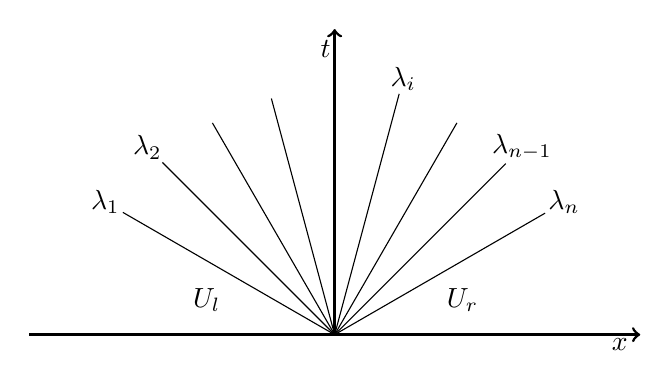
\begin{tikzpicture}[scale = {0.015\linewidth},inner sep = 1pt]
%% \begin{tikzpicture}[scale = {0.015\linewidth},inner sep = 1pt]
%% \tikzstyle{every node} = [draw,circle,fill=gray!30];
%% \draw (-1.5,0.0) circle (0.8);
%% \draw[<->,line width=1pt] (0,1) node[right]{\;$t$}|-(1,0) node[below]{$m$};
\draw[line width=1pt] (0,0.7) node[left]{$t$}|-(0.7,0) node[below]{$x$};
\draw[->,line width=1pt] (0.7,0)--(0.75,0);
\draw[->,line width=1pt] (0,0.7)--(0,0.75);  
\draw[line width=1pt] (0,0)--(-0.75,0);


\node[draw=white] (w1) at (-0.56292,0.32500) {$\lambda_1$};
\node[draw=white] (w2) at (-0.45962,0.45962) {$\lambda_2$};
\node[draw=white] (wi) at (0.16823,0.62785) {$\lambda_i$};
\node[draw=white] (w5) at (0.45962,0.45962) {$\lambda_{n-1}$};
\node[draw=white] (w6) at (0.56292,0.32500) {$\lambda_n$};

\node[draw=white] (ul) at (-0.31393,0.084116) {$\mbf{U}_l$};
\node[draw=white] (ur) at (0.31393,0.084116) {$\mbf{U}_r$};

%% \node[draw=white] (R8a) at (0.53943,0.10730) {\small $\mathrm{R}$8};
%% \node[draw=white] (R7a) at (0.45731,0.30556) {\small $\mathrm{R}$7};
%% \node[draw=white] (R6a) at (0.30556,0.45731) {\small $\mathrm{R}$6};
%% \node[draw=white] (R5a) at (0.10730,0.53943) {\small $\mathrm{R}$5};
%% \node[draw=white] (R4a) at (-0.10730,0.53943) {\small $\mathrm{R}$4};
%% \node[draw=white] (R3a) at (-0.30556,0.45731) {\small $\mathrm{R}$3};
%% \node[draw=white] (R2a) at (-0.45731,0.30556) {\small $\mathrm{R}$2};
%% \node[draw=white] (R1a) at (-0.53943,0.10730) {\small $\mathrm{R}$1};

%% \node[] at (0.15,0.95) {contact};
\draw (0,0) -- (w1);  
\draw (0,0) -- (w2);  
\draw (0,0) -- (-0.30000,0.51962);%(w3);  
\draw (0,0) -- (-0.15529,0.57956);
\draw (0,0) -- (wi);  
\draw (0,0) -- (0.30000,0.51962);%(w4);  
\draw (0,0) -- (w5);  
\draw (0,0) -- (w6);  
\end{tikzpicture}
